% ----------------------------------------- Sample ----------------------------------------

% \lipsum[61-80]


% ----------------------------------------- Real ----------------------------------------

\section{Motivation}
This section describes the approximations that are made and how certain considerations allow us to simplify the equations, by omitting terms that are known to be small or information that is not important.

The most important, and the most delicate, approximation is naturally the neglect of viscosity.
The coefficient of viscosity is small, but it multiplies the highest derivative, and the perturbation problem is said to be singular.
The inviscid problem and the viscous problem have very different characters; in particular they do not require the same number of boundary conditions.
Regions exist in the flow where the velocity gradients are so large that the viscous term is as large as the inertial term.
This viscous term can change the local value of the vorticity by an amount of order 1, meaning that it does not tend to zero while the coefficient of viscosity does.
Therefore the flow with small viscosity cannot be treated as slightly different from the inviscid flow in the usual sense, and a straightforward attempt to expand the solution as a power series in $\nu$ would fail.

The justification for omitting the viscosity is the following.
The effect of viscosity will be to diffuse the vorticity over very short distances, without creating or destroying any.
(The viscous term in Eq. ??? is the divergence of $\nu \grad \omega$, which is interpreted as a flux of vorticity. It is not source term.)
Let $L$ be the length scale associated with the body, $\Uinf$ the free stream velocity and $\nu$ the kinematic viscosity.
The non-dimensional number $L\Uinf/\nu$ is the Reynolds number, and is large in all cases under consideration.
The length scale associated with the viscous diffusion if $\sqrt{\nu t}$ where $t$ is the "age" of the vorticity.
Let us consider some vorticity which is "born" at the solid boundary and in a time $L/\Uinf$ is transported into the wake, to a distance $L$ from the solid.
The viscous scale becomes $\sqrt{\nu L/\Uinf}$ and the ratio of this scale to $L$ is $\sqrt{\nu/L\Uinf}$, or $Re^{-1/2}$, and thus is small.
In general the flow properties close to the solid boundary will not be sensitive to the displacement of the vorticity over such a small distance.
Since predicting the stresses on the solid is the ultimate objective of the study, omitting detailed information about the vorticity diffusion in the wake is minor as long as the transport is correct.

However the vorticity is "produced" at the solid boundary and its subsequent transport is very sensitive to its initial life, near the wall, during which the scales are small and the viscous term is important.
It is the convection with the fluid that carries the vorticity into the large structures of the wake, but the velocity is zero at the wall and only the viscosity can make the vorticity penetrate into the stream at all.
Therefore the "justification" we just reviewed breaks down in the wall region.

This motivates the procedure of coupling an invisicid outer flow and a viscous boundary layer flow.
This procedure is common when the outer flow is not only treated as inviscid but also as irrotational.
Here, the outer flow will be vertical.
The effort will be worthwhile if an efficient solver is available for the simplified equations in each region.

The vortex method is efficient in the outer flow; it treats the transport term accurately and provides the necessary resolution in the wake.
It does not cause any problem at large distances from the body.
Its weakness in treating the detailed viscous features will not disturb the large scale structures which dominate in the wake.
The implicit finite difference method is very good at treating thin viscous flows.
For such a small and logically rectangular domain it is also very fast.
Both methods are available and well tested.
The new element that is needed is a procedure that makes the two regions interact through the boundary conditions at the interface.

The systematic mathematical formulation of these ideas are presented in the following, and some comments about the method are then followed.


\section{Matched asymptotic analysis}

\begin{figure}
 \begin{center}
 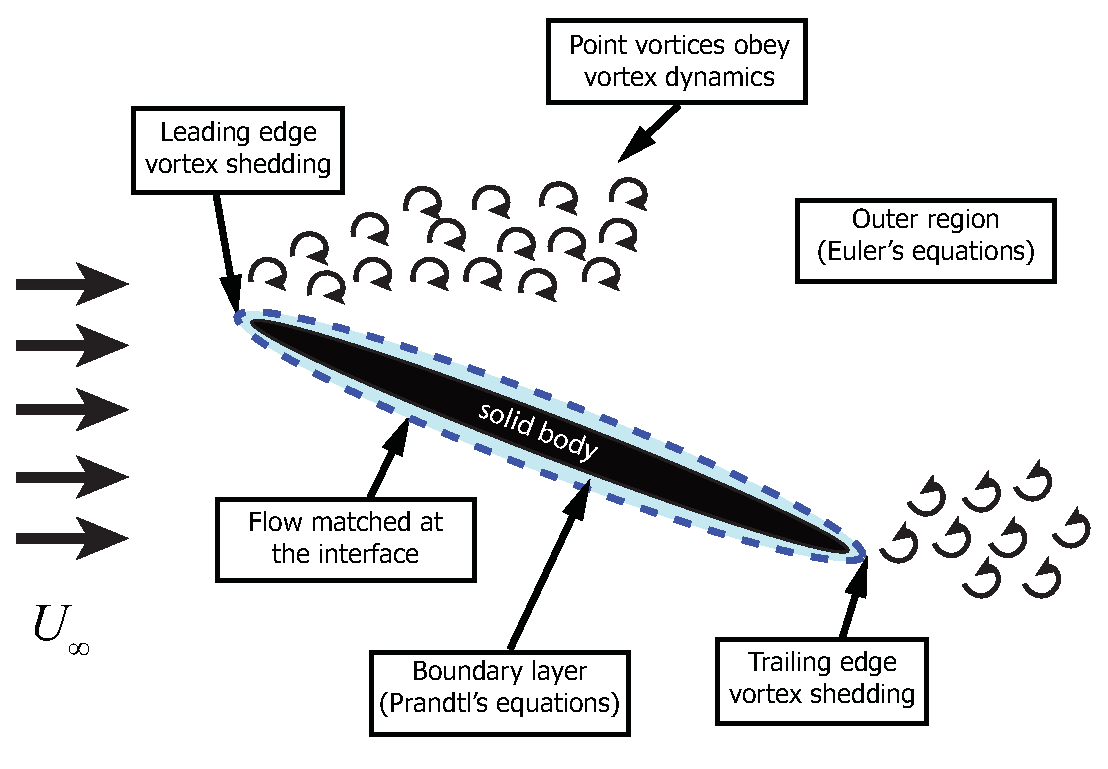
\includegraphics[width = 14cm]{./Figures/ModelSchematic.eps}
\end{center}
 \caption{A schematic description of the model}
 \label{fig:modelschematic}
\end{figure}

\subsection{Outer flow}

For high-Reynolds-number flow, the viscous term is dropped as mentioned before, and the governing equations are correspondingly the inviscid Euler's equations
\begin{align}
\bu_t + \bu \cdot \grad \bu  =  -\grad p,  \quad
\grad \cdot \bu  =  0.
\label{eqn:Euler}
\end{align}
One of the consequences of this simplification is that the order of the equations in space is reduced from 2 to 1, and the required number of boundary conditions is reduced correspondingly.
The boundary of this domain is composed of two parts, infinity and the interface $C$ with the boundary layer. 
At infinity, the natural choice of boundary condition is $\bu = \Uinf$, and the proper boundary condition on the interface $C$ will be discussed later.

\subsection{Inner flow}

The inviscid approximation above is valid except in the thin region close to the body, or the so-called boundary layer.
The boundary layer thickness scales as $\delta = c\sqrt{\nu}$, where $c$ is a dimensionless number of order $1$.
In the boundary layer the viscous term are retained, but the thinness of the layers renders some terms negligible.
Curvature effects will not be included.
This is legitimate for shapes like a circular cylinder; for airfoils, it might be necessary to account for curvature near the trailing edge, or to round it off so as to increase its radius of curvature.
The governing equations in this region are the classical Prandtl's approximation
\begin{align}
u_t + uu_{\theta} + vu_{\eta}  =  - \Pi_{\theta} + \visc u_{\eta\eta},  \quad
u_\theta + v_\eta  =  0,
\label{eqn:Prandtl}
\end{align}
in which ($\theta$,$\eta$) is the local coordinate system, ($u$,$v$) are the corresponding velocity components and $\Pi$($\theta$,$t$) denotes the pressure. 
On the surface of static solid body, they satisfy the same no penetration and no slip conditions $u = v = 0$.

\subsection{Coupling}

On the interface $C$ between the boundary layer and the outer region, we impose the continuity of velocity components, pressure and vorticity as
\begin{equation}
 u = \bu \cdot \bt, \quad v = \bu \cdot \bn,  \quad \Pi = p, \text{ and } u_{\eta} v = \omega \bu \cdot \bn,
\label{eqn:matchingbcs}
\end{equation}
where ($\bt$, $\bn$) are the local tangential and normal directions on $C$, and vorticity is defined as $\omega \bk = \grad \times \bu$. 
The last of these conditions is imposed only for outflow ($v = \bu \cdot \bn > 0$) and provides an estimate for the vorticity shed from the boundary layer to the outer region.


\section{Rationale}

Our method is based on the well-known approximations to Navier-Stokes equations for high $\Rey$ where the viscous effects are dominated by inertia of the fluid everywhere except in a boundary layer of thickness scale $\visc^{1/2}$. 
Traditionally, these equations are arrived at by using matched asymptotic expansion, and require matching the flow field in an intermediate region.
In our model, we seek to replace the matching procedure with simple continuity conditions on a well-defined boundary curve $C$ between the two regions.
The nature of these conditions, are determined by considerations of matching the asymptotic solutions and simultaneously by the need for the approximate PDEs on both regions to be well-posed and possess unique solution.
We elaborate on these considerations below.

The velocity field in the outer inviscid region can be decomposed into a rotational component $\bu_{\omega}$ and a potential component $\grad \phi$ as $\bu = \bu_{\omega} + \grad \phi$, such that $\bu_\omega\to 0$ at infinity.
Then the incompressible condition requires that $\grad \phi$ satisfy the Laplace's equation
\begin{align}
\label{eqn:Laplace}
\grad^2 \phi = 0,
\end{align}
and $\bu_\omega$ is related to the vorticity field as
\begin{align}
\omega \bk = \grad \times \bu = \grad \times \bu_{\omega},
\end{align}
the inverse of which, under the condition of no flow at infinity, is given by the Biot-Savart law as
\begin{align}
\label{eqn:Biot-Savart}
\bu_{\omega} (\bx, t) =  \frac{1}{2\pi} \int_{S} d\by \frac{\omega(\by, t)\bk \times (\bx - \by)}{|\bx - \by|^2}.
\end{align}
Due to the inviscid dynamics in this region, the vorticity is merely advected with fluid elements satisfying
\begin{align}
 \omega_t + \bu\cdot\grad\omega = 0. \label{eqn:Vorticity}
\end{align}
The appropriate auxiliary conditions with this equation are the initial condition for vorticity $\omega$ and its flux across the boundary $C$, because of the hyperbolic nature of this equation. 
Similarly, because of the elliptic nature of \eqref{eqn:Laplace}, boundary data needs to be specified for $\phi$ (Dirichlet) or $\grad \phi \cdot \bn$ (Neumann) on $C$ and at $\infty$.
In our case, the specification of the normal velocity $\bu \cdot \bn$ on $C$, provides the Neumann boundary condition through $(\bu_\omega + \grad \phi) \cdot \bn = \bu \cdot \bn$.

In the boundary layer, similar considerations lead to our choice of boundary conditions.
The governing equations \eqref{eqn:Prandtl} are parabolic for $u$ in $\eta$ direction and hyperbolic in $\theta$ and $t$, while for $v$ they are hyperbolic. 
This indicates that the no-penetration condition on the body surface is enough to determine $v$, while for $u$ one extra condition is required on $C$ other than the no-slip condition on body surface. 
Besides, one boundary condition is required to determine pressure $\Pi$, typically on $C$.
Combining these considerations together, the conditions (???) provide the correct number and kind of conditions for (???) to be well-posed. 

The solution of the model is not expected to significantly depend on the precise location of the boundary curve $C$.
When going farther away from the body surface within the boundary layer, the solution of Prandtl's equation has an asymptote $u = $ const in normal direction $\eta$ (except the small region close to the separation point).
Physically, the viscous stress becomes smaller and smaller, and the advection of vorticity becomes more and more dominant over the diffusion effect.
This asymptotic behavior automatically matches with the inviscid behavior in the outer region for some appropriately matched pressure.
Mathematically, this expectation is strengthened by the fact that Prandtl's equation (???) degrades to the inviscid Euler equation (???) under the condition $u_\eta = 0$ and $\Pi = p$.
Therefore, the exact location of the boundary only determines the location where we switch over our representation from one form to the other, but the underlying flow remains the same.

Prandtl's boundary layer approximation is considered to be inapplicable near the region where the boundary layer separates. 
While a general asymptotic model of strongly coupled flow at high Reynolds number near separation point is not available, potential flow around a corner is considered a useful candidate for representing the outer region flow in the vicinity of separation (cite Meyer's review).
Near a corner of internal angle $\alpha$, the complex velocity potential is $U (z/L)^{\pi/\alpha}$, with velocity scaled as $U (z/L)^{\pi/\alpha-1}$.
If the length scale of the corner is assumed as $l \sim \visc^p L$ ($p > 0$), the velocity equation, scaled as $l/T \sim U(l/L)^{\pi/\alpha-1}$, gives the time scale in the corner as $T \sim \frac{L}{U} \visc^{p(2-\pi/\alpha)}$. 
In our case, from the upstream side $\alpha > \pi/2$, so the time scale $T$ near separation point is much smaller than the convection time scale $L/U$ with $\visc \ll 1$, which says the vorticity will leave the separation region once they get convected or created there and never get accumulated significantly. 
From the downstream side, the time scale is not small and vorticity gets accumulated; this is consistent with the cumulation of vorticity in the recirculation region downstream of the separation.
Therefore despite of this unavailability of an accurate model near separation point, the rate of vorticity shedding may not depend on the details of the flow near the point of separation, even when the flow is unsteady. 
We use the example of the impulsively started cylinder to verify this assumption.
